\documentclass{beamer}
%\setbeamersize{text margin left=30mm,text margin right=30mm} 
%\setbeamertemplate{frametitle}{\vspace{2cm} \\ \insertframetitle }
%\setbeamertemplate{footline}{\vspace{0.5cm}}
%\addtolength{\headsep}{-16cm}



% The Beamer class comes with a number of default slide themes
% which change the colors and layouts of slides. Below this is a list
% of all the themes, uncomment each in turn to see what they look like.
\mode<presentation> {
% \usetheme{Marburg}
% \usetheme{Singapore}
\usetheme{Montpellier}
% \usetheme{Ilmenau}
% \usetheme{Warsaw}
% \usecolortheme{orchid}
}
%\addtobeamertemplate{beamercolorbox}{}{\vspace{-20em}}

%\usepackage{bbm}

\usepackage[english]{babel}
\usepackage[utf8]{inputenc}
\usepackage[T1]{fontenc}

\usepackage[round]{natbib}
\usepackage{afterpage}
\usepackage{amsfonts}
\usepackage{amsmath}
\usepackage{amssymb}
\usepackage{amsthm}
\usepackage{array}
\usepackage{authblk}
\usepackage{booktabs}
\usepackage{caption}
\usepackage{color}
\usepackage{comment}
\usepackage{dcolumn}
\usepackage{enumitem}
\usepackage{epigraph}
\usepackage{epsfig}
\usepackage{epstopdf}
\usepackage{eurosym}
\usepackage{fancyhdr}
\usepackage{float}
%%%%%%%%%%%%%%%%%
\usepackage{footmisc}
\usepackage{geometry}
\usepackage{graphics}
\usepackage{graphicx} %\usepackage[graphicx]{realboxes}
\usepackage{indentfirst}
\usepackage{lipsum}
\usepackage{listings}
\usepackage{lmodern}
\usepackage{longtable}
\usepackage{lscape}
\usepackage{mathrsfs}
\usepackage{mathtools}
\usepackage{multirow}
\usepackage{pdflscape}
\usepackage{pgfplots}
\usepackage{placeins}
\usepackage{qtree}
\usepackage{rotating,tabularx}
\usepackage{setspace}
\usepackage{subfigure}
\usepackage{textcomp}
% \usepackage{titlesec}
% \usepackage{titletoc}%,minitoc
\usepackage{ulem}
\usepackage{verbatim}
\usepackage{xspace}
\usepackage{xtab}
%%%%%%%%%%%%%%%%%%%%%%%%%%%%%%%%%%%%%%%%%
\usepackage{tikz}
\usetikzlibrary{decorations.pathreplacing}
\usetikzlibrary{shapes}
\usetikzlibrary{spy,arrows,positioning,shapes.multipart}
\def\checkmark{\tikz\fill[scale=0.4](0,.35) -- (.25,0) -- (1,.7) -- (.25,.15) -- cycle;}
\usetikzlibrary{calc, automata, chains, arrows.meta}

\usepackage{xcolor}
\hypersetup{
colorlinks,
linkcolor={blue!50!black},
citecolor={blue!50!black},
urlcolor={blue!50!black}}


\newtheorem{proposition}{Proposition}
\newtheorem{axiom}{Axiom}
\newcommand{\ra}[1]{\renewcommand{\arraystretch}{#1}}

\newcommand{\E}{\mathrm{E}}
\newcommand{\Var}{\mathrm{Var}}
\newcommand{\Corr}{\mathrm{Corr}}
\newcommand{\Cov}{\mathrm{Cov}}

\newcolumntype{d}[1]{D{.}{.}{#1}} % "decimal" column type
\renewcommand{\ast}{{}^{\textstyle *}} % for raised "asterisks"

\newtheorem{hyp}{Hypothesis}
\newtheorem{subhyp}{Hypothesis}[hyp]
\renewcommand{\thesubhyp}{\thehyp\alph{subhyp}}

\newcommand{\red}[1]{{\color{red} #1}}
\newcommand{\blue}[1]{{\color{blue} #1}}

%\newcommand*{\qed}{\hfill\ensuremath{\blacksquare}}%

\newcolumntype{L}[1]{>{\raggedright\let\newline\\arraybackslash\hspace{0pt}}m{#1}}
\newcolumntype{C}[1]{>{\centering\let\newline\\arraybackslash\hspace{0pt}}m{#1}}
\newcolumntype{R}[1]{>{\raggedleft\let\newline\\arraybackslash\hspace{0pt}}m{#1}}

%\geometry{left=1.5in,right=1.5in,top=1.5in,bottom=1.5in}
%\geometry{left=1in,right=1in,top=1in,bottom=1in}

\epstopdfsetup{outdir=./}

\newcommand{\elabel}[1]{\label{eq:#1}}
\newcommand{\eref}[1]{Eq.~(\ref{eq:#1})}
\newcommand{\ceref}[2]{(\ref{eq:#1}#2)}
\newcommand{\Eref}[1]{Equation~(\ref{eq:#1})}
\newcommand{\erefs}[2]{Eqs.~(\ref{eq:#1}--\ref{eq:#2})}

\newcommand{\Sref}[1]{Section~\ref{sec:#1}}
\newcommand{\sref}[1]{Sec.~\ref{sec:#1}}

\newcommand{\Pref}[1]{Proposition~\ref{prop:#1}}
\newcommand{\pref}[1]{Prop.~\ref{prop:#1}}
\newcommand{\preflong}[1]{proposition~\ref{prop:#1}}

\newcommand{\Aref}[1]{Axiom~\ref{ax:#1}}

\newcommand{\clabel}[1]{\label{coro:#1}}
\newcommand{\Cref}[1]{Corollary~\ref{coro:#1}}
\newcommand{\cref}[1]{Cor.~\ref{coro:#1}}
\newcommand{\creflong}[1]{corollary~\ref{coro:#1}}

\newcommand{\etal}{{\it et~al.}\xspace}
\newcommand{\ie}{{\it i.e.}\ }
\newcommand{\eg}{{\it e.g.}\ }
\newcommand{\etc}{{\it etc.}\ }
\newcommand{\cf}{{\it c.f.}\ }
\newcommand{\ave}[1]{\left\langle#1 \right\rangle}
\newcommand{\person}[1]{{\it \sc #1}}

\newcommand{\AAA}[1]{\red{{\it AA: #1 AA}}}
\newcommand{\YB}[1]{\blue{{\it YB: #1 YB}}}

\newcommand{\flabel}[1]{\label{fig:#1}}
\newcommand{\fref}[1]{Fig.~\ref{fig:#1}}
\newcommand{\Fref}[1]{Figure~\ref{fig:#1}}

\newcommand{\tlabel}[1]{\label{tab:#1}}
\newcommand{\tref}[1]{Tab.~\ref{tab:#1}}
\newcommand{\Tref}[1]{Table~\ref{tab:#1}}

\newcommand{\be}{\begin{equation}}
\newcommand{\ee}{\end{equation}}
\newcommand{\bea}{\begin{eqnarray}}
\newcommand{\eea}{\end{eqnarray}}

\newcommand{\bi}{\begin{itemize}}
\newcommand{\ei}{\end{itemize}}

\newcommand{\Dt}{\Delta t}
\newcommand{\Dx}{\Delta x}
\newcommand{\Epsilon}{\mathcal{E}}
\newcommand{\etau}{\tau^\text{eqm}}
\newcommand{\wtau}{\widetilde{\tau}}
\newcommand{\xN}{\ave{x}_N}
\newcommand{\Sdata}{S^{\text{data}}}
\newcommand{\Smodel}{S^{\text{model}}}

\newcommand{\del}{D}
\newcommand{\hor}{H}

\setlength{\parindent}{0.0cm}
\setlength{\parskip}{0.4em}

\numberwithin{equation}{section}
\DeclareMathOperator\erf{erf}
%\let\endtitlepage\relax

\AtBeginSection[]{
  \begin{frame}
  \vfill
  \centering
  \begin{beamercolorbox}[sep=8pt,center,shadow=true,rounded=true]{title}
    \usebeamerfont{title}\insertsectionhead\par%
  \end{beamercolorbox}
  \vfill
  \end{frame}
}


%\mode<presentation> {

% The Beamer class comes with a number of default slide themes
% which change the colors and layouts of slides. Below this is a list
% of all the themes, uncomment each in turn to see what they look like.

% As well as themes, the Beamer class has a number of color themes
% for any slide theme. Uncomment each of these in turn to see how it
% changes the colors of your current slide theme.

%\usecolortheme{albatross}
%\usecolortheme{beaver}
%\usecolortheme{beetle}
%\usecolortheme{crane}
%\usecolortheme{dolphin}
%\usecolortheme{dove}
%\usecolortheme{fly}
%\usecolortheme{lily}
%\usecolortheme{orchid}
%\usecolortheme{rose}
%\usecolortheme{seagull}
%\usecolortheme{seahorse}
%\usecolortheme{whale}
%\usecolortheme{wolverine}

%\setbeamertemplate{footline} % To remove the footer line in all slides uncomment this line
%\setbeamertemplate{footline}[page number] % To replace the footer line in all slides with a simple slide count uncomment this line


%----------------------------------------------------------------------------------------
%	TITLE PAGE
%----------------------------------------------------------------------------------------

\title[Innovation and choice]{Innovation and choice} % The short title appears at the bottom of every slide, the full title is only on the title page

\author{ Diomides Mavroyiannis, } % Your name
\institute[Dauphine] % Your institution as it will appear on the bottom of every slide, may be shorthand to save space
{
PSL/Paris Dauphine \\ % Your institution for the title page
\medskip% Your email address
}
\date{\today} % Date, can be changed to a custom date

\begin{document}

\begin{frame}
\titlepage % Print the title page as the first slide
\end{frame}

% \begin{frame}{Overview}
% \tableofcontents
% \end{frame}

% \begin{frame}{Jury members}
% \begin{itemize}
%     \item Olivier Bos, Rapporteur
%     \item Sara Biancini, Rapporteur
%     \item Frederic Loss, Examinateur
%     \item Claire Chambolle, Examinateur
%     \item David Ettinger, Directeur de thèse 
% \end{itemize}
% \end{frame}

\begin{frame}{General motivation}
\begin{itemize}
    \item What is an innovation? New market or increase surplus in existing market
%    \item There is some project that will be undertaken if its costs exceed its benefits. There are many reasons why this would not occur, the language of economics likes to frame these frictions as transaction costs. 
% \item Innovation would present no problem if contracting was possible everywhere. 
    \item The problem of ex-ante contractability. (Incomplete Contracts, Grossman and Hart(1986))
%If firms cannot contract before an innovation exists, there exists a problem of 
    \item Solution: Intellectual property, endogenize research, etc
% \item if the innovation isn't ex-ante profitable, why would we want to pursue it? 
% \item The problem is the disconnect between profits and welfare, maybe an innovation will be worthwhile from the point of view of welfare but not from the point of view of profits. 
% \item the problem of fixed research/development costs. 
\end{itemize}
\end{frame}

% \begin{frame}
% \begin{figure}
% \resizebox{11cm}{7cm}{
% \centering
% %\begin{tikzpicture}[every text node part/.style={align=center}] used for multiple parts,
% %along with shapes.multipart tikz library.
% \begin{tikzpicture}[sharp corners=2pt,inner sep=7pt,node distance=.8cm,every text node part/.style={align=center}]
% \node[draw, minimum height = 3cm, minimum width = 3cm](Privilege){\textbf{Privilege:} A can use \\ \textcolor{blue}{ \textbf{Power:} A can change B's  rights}};
% \node[draw, below=2cm of Privilege, minimum height = 3cm, minimum width = 3cm](Duty){\textbf{Duty:} A has no right to use \\ \textcolor{blue}{\textbf{Disability:} A can't change B's rights}};
% \node[draw,right=2cm of Privilege, minimum height = 3cm, minimum width = 3cm](No-claim){\textbf{No-claim:} B cannot exclude A\\ \textcolor{blue}{\textbf{Liability:} B's rights can be changed by A}};
% \node[draw,below=2cm of No-claim, minimum height = 3cm, minimum width = 3cm](Claim){\textbf{Claim:} B can exclude A \\ \textcolor{blue}{\textbf{Immunity:} B's rights can't be changed by A}};

% %Draw arrows
% \draw[-triangle 90, ultra thick,<->] (Privilege) -- (Duty) node [midway, above, left = 0.1cm]{opposite:};
% \draw[-triangle 90, ultra thick,<->] (Privilege) -- (No-claim) node [midway, above]{correlative:};
% \draw[-triangle 90, ultra thick,<->] (No-claim) -- (Claim) node [midway, above, right = 0.1cm]{opposite: };
% \draw[-triangle 90, ultra thick,<->] (Duty) -- (Claim) node [midway, above]{correlative:};
% %\draw[-triangle 90, ultra thick,<->] (Privilege) -- (Claim) node [midway, above, rotate = -45]{$\mu^{03}_{x+t:y+t}$};
% \end{tikzpicture}}
% \caption{First order rights, \textcolor{blue}{Second order rights}}
% \end{figure}
% \end{frame}


\begin{frame}{Structure}
\begin{itemize}
    \item First chapter: What occurs when a single firm has a monopoly on a good which has social value? 
    \item Second chapter: How does the option of a firm to be acquired change its innovation choices?
    \item Third chapter: We explore the causes of discounting
% \item if the innovation isn't ex-ante profitable, why would we want to pursue it? 
% \item The problem is the disconnect between profits and welfare, maybe an innovation will be worthwhile from the point of view of welfare but not from the point of view of profits. 
% \item the problem of fixed research/development costs. 
% \item  
\end{itemize}
\end{frame}

% \setcounter{tocdepth}{1}
\section{Chapter 1: Piracy and network value}
%%%%%%%%%%%%%%%%%%%%%%%%%%%%%%%%%%%%
%%%%%%%%%%%%%%%%%%%%%%%%%%%%%%%%%%%%
%%%%%%%%%%%%%%%%%%%%%%%%%%%%%%%%%%%%
\begin{frame}{Motivation: Piracy}
\begin{itemize}
    \item The intellectual property claim: limiting entry $\rightarrow$ increases the incentive to innovate.
    \item The piracy claim: making piracy illegal $\rightarrow$ increases the incentive to innovate.
    \item The monopoly issue: If a single firm sells the asset and has control of the price $\rightarrow$ the price set will be above what is welfare maximizing. 
\end{itemize}
\end{frame}
%%%%%%%%%%%%%%%%%%%%%%%%%%%%%%%%%%%%
\begin{frame}{Questions}
\begin{itemize}
    \item 1) Does uniform enforcement of intellectual property increase innovation?
    \item 2) Does social value enchance or curtail monopoly power?
    \item 3) Who benefits from piracy? 
    \item 4) Is the incentive to improve the product independent of social value? 
\end{itemize}
\end{frame}
%%%%%%%%%%%%%%%%%%%%%%%%%%%%%%%%%%%%
\begin{frame}{Model components:}
\begin{itemize}
%Legal Assymetry 
%     \item When a firm violates a copyright it is an infringment (tort) 
%     \item When a consumer violates a copyright it is theft (criminal)
% % The cost of pirating is set exogenously whilst the cost of infringement is set endogenously
% % Is there a time where a firm does not wish to enforce it's right? 
%     \item Digital goods have only fixed costs, marginal costs are zero
    \item The main modelling component used is social value.
    \item Agents have the option of buying, pirating and not using.
    \item Using encompasses pirating or buying. 
    \item Easier to pirate 
        \begin{itemize}
            \item  $\rightarrow$ More pirates some of which used to buy but also higher willingness to pay of buyers. 
            \item  $\rightarrow$ Buyers have a higher willingness to pay.
        \end{itemize}
\end{itemize}
\end{frame}
%%%%%%%%%%%%%%%%%%%%%%%%%%%%%%%%%%%%
\begin{frame}{Tentative answer 1}
\begin{itemize}
    \item Does uniform enforcement of intellectual property increase innovation? \textcolor{red}{No}
    \item \textcolor{orange}{Causal Mechanism:} \textcolor{blue}{Piracy can increase profits.}
\end{itemize}
\end{frame}
%%%%%%%%%%%%%%%%%%%%%%%%%%%%%%%%%%%%
\begin{frame}{Tentative answer 2}
\begin{itemize}
    \item Does social value enhance or curtail monopoly power? \textcolor{red}{curtail}
    \item \textcolor{orange}{Causal Mechanism:} \textcolor{blue}{Number of agents consuming increases $\rightarrow$ Product value increases $\rightarrow$ Monopolist will try to increase users.}
\end{itemize}
\end{frame}
%%%%%%%%%%%%%%%%%%%%%%%%%%%%%%%%%%%%
\begin{frame}{Tentative answer 3}
\begin{itemize}
    \item Who benefits from piracy?  \textcolor{red}{Consumers with a lower willingness to pay will benefit. Firms may benefit.}
    \item \textcolor{orange}{Causal Mechanism:} \textcolor{blue}{Firms may benefit by including lower willingness to pay agents by charging higher willingness to pay agents more.}
\end{itemize}
\end{frame}
%%%%%%%%%%%%%%%%%%%%%%%%%%%%%%%%%%%%
\begin{frame}{Tentative answer 4}
\begin{itemize}
    \item Is the incentive to improve the product independent of network value? \textcolor{red}{No}
    \item \textcolor{orange}{Causal Mechanism:} \textcolor{blue}{A high network value may be a substitute to innovation.}
\end{itemize}
\end{frame}
%%%%%%%%%%%%%%%%%%%%%%%%%%%%%%%%%%%%
\section{Chapter 2: Cost side innovation with project variance}
%%%%%%%%%%%%%%%%%%%%%%%%%%%%%%%%%%%%
%%%%%%%%%%%%%%%%%%%%%%%%%%%%%%%%%%%%
\begin{frame}{Motivation}
\begin{itemize}
    \item Buyouts claim: Having the option of being bought out can only increase innovation. 
    \item Industry consolidation: Is it efficienct?
\end{itemize}
\end{frame}
%%%%%%%%%%%%%%%%%%%%%%%%%%%%%%%%%%%%
\begin{frame}{Questions}
\begin{itemize}
    \item 1) Does the alienability of assets have a uniform effect (is the order the same)?
    \item $B<A<0 \rightarrow 0<B<A $
    \item $B<A<0 \rightarrow 0<A<B $  
% So suppose two projects have a value of 100 without buyouts, do both projects have a value of 150 with buyouts?  
    \item 2) Do existing firms always have an incentive to promote buyouts?
    \item 3) Why does successful innovation often lead to buyouts?
% Why do so many entrepreneurs end up being bought over? 
\end{itemize}
\end{frame}


\begin{frame}{Modelling structure}
Incumbent is ahead, entrant can choose project 
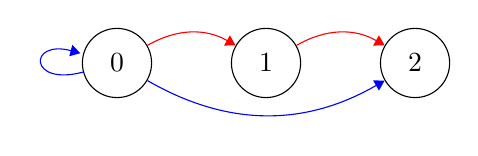
\begin{tikzpicture}[start chain = going right,
   -Triangle, every loop/.append style = {-Triangle}]
   \foreach \i in {0,...,2} 
     \node[state, on chain]  (\i) {\i};
   \foreach \i in {0,1} {
     \draw[red] let \n1 = { int(\i+1) } in
       (\i)  edge[bend left] (\n1);
   }
   \draw[blue] (0) edge[bend right] (2);
   \draw[blue] (0) edge[loop left] (0);
   % \foreach \i in {1,...,3}
   %   \draw  (\i) edge[loop below] (\i);
   % \draw    (0)  edge[loop left]   (0);
   % \draw    (4)  edge[loop right]  (4);
\end{tikzpicture}
\end{frame}
%%%%%%%%%%%%%%%%%%%%%%%%%%%%%%%%%%%%
%%%%%%%%%%%%%%%%%%%%%%%%%%%%%%%%%%%%
\begin{frame}{Tentative answer 1}
\begin{itemize}
    \item Does the alienability of assets have a uniform effect (is the order the same)? \textcolor{red}{No}
    \item \textcolor{orange}{Causal Mechanism:} \textcolor{blue}{The entrant can monetize damage done to the incumbent with the intermediate technology.}
\end{itemize}
\end{frame}
%%%%%%%%%%%%%%%%%%%%%%%%%%%%%%%%%%%%
\begin{frame}{Tentative answer 2}
\begin{itemize}
    \item Do existing firms always have an incentive to promote buyouts? \textcolor{red}{No}
    \item \textcolor{orange}{Causal Mechanism:} \textcolor{blue}{Not regulating mergers can lead to a situation where blackmail occurs. Entrants pursue damage maximizing projects instead of profit maximizing.}
\end{itemize}
\end{frame}
%%%%%%%%%%%%%%%%%%%%%%%%%%%%%%%%%%%%
\begin{frame}{Tentative answer 3}
\begin{itemize}
    \item Why does successful innovation often lead to buyouts?\textcolor{red}{ Because innovators purposefully choose projects with the intent of being bought out.}
    \item \textcolor{orange}{Causal Mechanism:} \textcolor{blue}{Entrants will prefer correlated projects}
\end{itemize}
\end{frame}
%%%%%%%%%%%%%%%%%%%%%%%%%%%%%%%%%%%%

    % \item The longer the time horizon, the lower the distortion effect

%%%%%%%%%%%%%%%%%%%%%%%%%%%%%%%%%%%%
\section{Chapter 3: Microfoundations of Discounting}
%%%%%%%%%%%%%%%%%%%%%%%%%%%%%%%%%%%%
%%%%%%%%%%%%%%%%%%%%%%%%%%%%%%%%%%%%
% \begin{frame}{The problem situation: What do agents do?}
% \begin{figure}[!htb]
% \centering
% 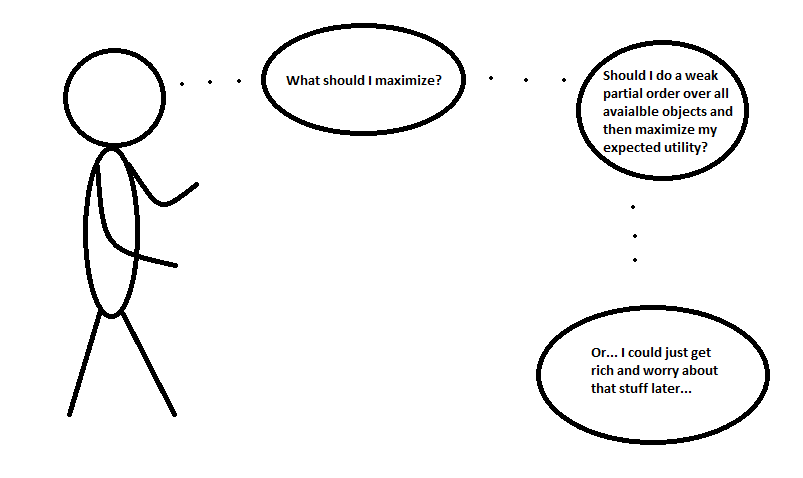
\includegraphics[width=1.0\textwidth]{./figures/maximize.PNG}
% \caption{What to do?}
% \flabel{caseA}
% \end{figure}
% \end{frame}
\begin{frame}{Discounting: motivation}
\begin{itemize}
    \item \textbf{Phenomenon:} Agents prefer present payments to future payments. 
    \item \textbf{Definition:} A discount rate is the rate you must multiply the future payment to get the value of an equivalent payment in the present.
    \item Experimentally, people discount payment hyperbolically, yet there is variance.
    \item Firm criteria for investing is mostly based on exponential discounting (NPV).
    \item Theory points to exponential discounting as profit maximizing.
    % \item "Preferences" is used as an explanatory tool to reconcile exponential and hyperbolic
\end{itemize}
\end{frame}


\begin{frame}
\begin{figure}[!htb]
\resizebox{11cm}{7cm}{
\centering
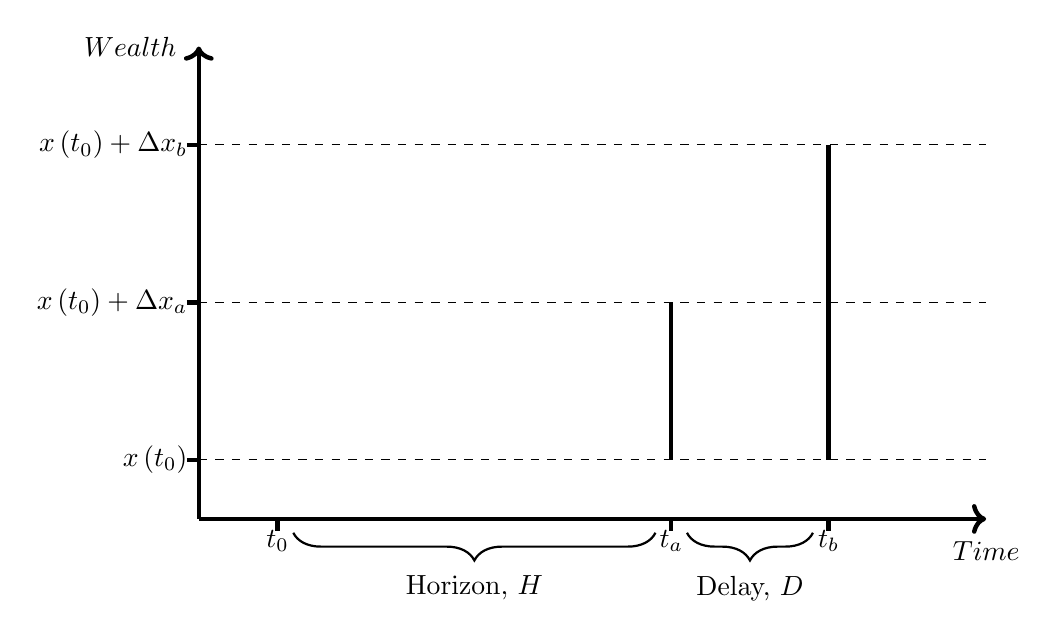
\begin{tikzpicture}
%\draw[help lines, color=gray!30, dashed] (-5,0) grid (4.9,5.9);
\draw[->,ultra thick] (-5,0)--(5,0) node[below,yshift=-4pt]{$Time$};
\draw[->,ultra thick] (-5,0)--(-5,6) node[left,xshift=-4pt]{$Wealth$};
\draw[-,ultra thick] (-4,-0.15)--(-4,0) node[below]{$t_0$};
\draw[-,ultra thick] (1,-0.15)--(1,0) node[below]{$t_a$};
\draw[-,ultra thick] (3,-0.15)--(3,0) node[below]{$t_b$};
\draw[-,ultra thick] (-5.15,0.75)--(-5,0.75) node[left]{$x\left(t_0\right)$};
\draw[-,ultra thick] (-5.15,2.75)--(-5,2.75) node[left]{$x\left(t_0\right) + \Dx_a$};
\draw[-,ultra thick] (-5.15,4.75)--(-5,4.75) node[left]{$x\left(t_0\right) + \Dx_b$};
\draw[-, dashed] (-5,0.75)--(5,0.75) ;
\draw[-, dashed] (-5,2.75)--(5,2.75) ;
\draw[-, dashed] (-5,4.75)--(5,4.75) ;
\draw[-, ultra thick] (1,0.75)--(1,2.75) ;
\draw[-, ultra thick] (3,0.75)--(3,4.75) ;
\draw [decorate,decoration={brace,amplitude=10pt,mirror},xshift=0pt,yshift=-5pt,thick](-3.8,0) -- (0.8,0) node [black,midway,yshift=-20pt]{$\text{Horizon, }\hor$};
\draw [decorate,decoration={brace,amplitude=10pt,mirror},xshift=0pt,yshift=-5pt,thick](1.2,0) -- (2.8,0) node [black,midway,yshift=-20pt]{$\text{Delay, }\del$};
\end{tikzpicture} }
% \caption{The basic setup of the model. A decision maker faces a choice at time $t_0$ between option $a$, which guarantees a payment of $\Dx_a$ at time $t_a$, and option $b$, which guarantees a payment of $\Dx_b>\Dx_a$ at time $t_b>t_a$. We define the time between the decision and the earlier payment as the {\it horizon}, $\hor\equiv t_a-t_0$; and the time between the two payments as the {\it delay}, $\del\equiv t_b-t_a$.}
\flabel{basicsetup}
\end{figure}
\end{frame}

%%%%%%%%%%%%%%%%%%%%%%%%%%%%%%%%%%%%
%%%%%%%%%%%%%%%%%%%%%%%%%%%%%%%%%%%%
% \begin{frame}{The problem situation: What do agents do?}
% \begin{figure}[!htb]
% \centering
% 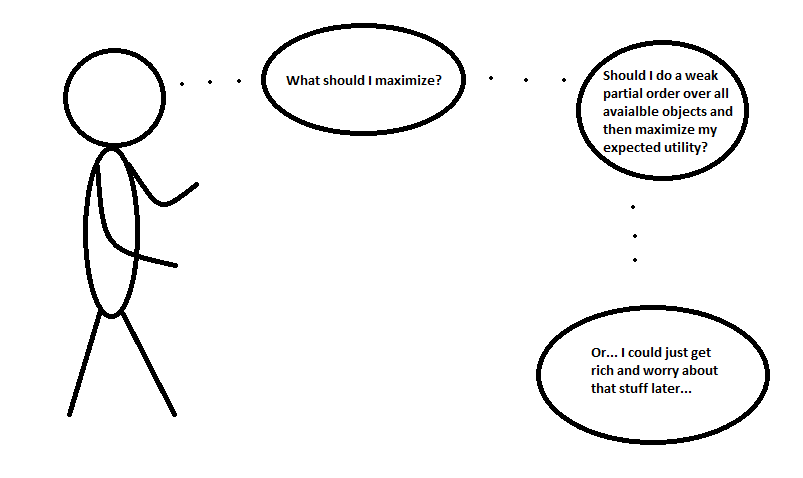
\includegraphics[width=1.0\textwidth]{./figures/maximize.PNG}
% \caption{What to do?}
% \flabel{caseA}
% \end{figure}
% \end{frame}
%%%%%%%%%%%%%%%%%%%%%%%%%%%%%%%%%%%%

%%%%%%%%%%%%%%%%%%%%%%%%%%%%%%%%%%%%
%%%%%%%%%%%%%%%%%%%%%%%%%%%%%%%%%%%%
% \begin{frame}{The pros and cons of preferences}
% \begin{itemize}
%     \item \textcolor{green}{Pro:} If we can characterize an agents preferences, we can predict an agents conditional behavior. 
%     \item \textcolor{red}{Con:} We cannot explain why agent A and B have different preferences
% \end{itemize}
% \end{frame}
%%%%%%%%%%%%%%%%%%%%%%%%%%%%%%%%%%%%
\begin{frame}{An alternative to preferences: Adaptation}
\begin{itemize}
    \item Economics: Preferences + Environment $\rightarrow$ Strategy
    \item Biology: Environment $\rightarrow$ Preferences/Strategy 
    \item Preferences are adaptations, if it were conscious it would be a strategy. 
\end{itemize}
\end{frame}
%%%%%%%%%%%%%%%%%%%%%%%%%%%%%%%%%%%%
%%%%%%%%%%%%%%%%%%%%%%%%%%%%%%%%%%%%
\begin{frame}{Questions}
\begin{itemize}
    \item 1) Why do agents have different ways of discounting?
    \item 2) How do we reconcile the normative method of discounting (exponential) and the descriptive method (hyperbolic)?
    \item 3) Can we draw out new falsifiable predictions from a unified framework? 
\end{itemize}
\end{frame}
%%%%%%%%%%%%%%%%%%%%%%%%%%%%%%%%%%%%
%%%%%%%%%%%%%%%%%%%%%%%%%%%%%%%%%%%%
%%%%%%%%%%%%%%%%%%%%%%%%%%%%%%%%%%%%
\begin{frame}{Some modelling choices used:}
\begin{itemize}
    \item Base assumption: Maximize growth of wealth.
    \item Multiplicative vs additive.
% People prefer more wealth to less wealth
    \item Some choices can affect future choices.
    \item Agents have different wealth levels.
    \item $\rightarrow$ Can imply that exponential discounting is not always the best way to maximize profits/wealth.
\end{itemize}
\end{frame}
%%%%%%%%%%%%%%%%%%%%%%%%%%%%%%%%%%%%
%%%%%%%%%%%%%%%%%%%%%%%%%%%%%%%%%%%%
%%%%%%%%%%%%%%%%%%%%%%%%%%%%%%%%%%%%
%%%%%%%%%%%%%%%%%%%%%%%%%%%%%%%%%%%%
\begin{frame}{Tentative answer 1}
\begin{itemize}
    \item Why do agents have different ways of discounting?\textcolor{red}{ Agents discount as a function of their different environments.}
    \item \textcolor{orange}{Causal Mechanism:} \textcolor{blue}{Growth depends on the kind of process that the agents face, which means their heterogeneity can be explained by the variation in their environment.}
\end{itemize}
\end{frame}
%%%%%%%%%%%%%%%%%%%%%%%%%%%%%%%%%%%%
%%%%%%%%%%%%%%%%%%%%%%%%%%%%%%%%%%%%
\begin{frame}{Tentative answer 2}
\begin{itemize}
    \item How do we reconcile the normative method of discounting (exponential) and the descriptive method (hyperbolic)? \textcolor{red}{It depends on the agents time horizon and growth process.}
    \item \textcolor{orange}{Causal Mechanism:} \textcolor{blue}{
    \item Multiplicative + Fixed = Exponential
    \item Additive + Adaptive = Hyperbolic}
\end{itemize}
\end{frame}
%%%%%%%%%%%%%%%%%%%%%%%%%%%%%%%%%%%%
%%%%%%%%%%%%%%%%%%%%%%%%%%%%%%%%%%%%
\begin{frame}{Tentative answer 3}
\begin{itemize}
    \item Can we draw out new falsifiable predictions from a unified framework? \textcolor{red}{Yes}
    \item \textcolor{orange}{Causal Mechanism:} \textcolor{blue}{
    \item Additive + Fixed = Highest payout $\rightarrow$ unconstrained capacity and unscaleable project based firms don't discount
    \item Multiplicative + Adaptive = Hybrid $\rightarrow$ firms with constrained capacity with projects that depend on scale discount the most
    \item $\rightarrow$ Wealth of agents can affect their discounting. } 
\end{itemize}
\end{frame}

\begin{frame}
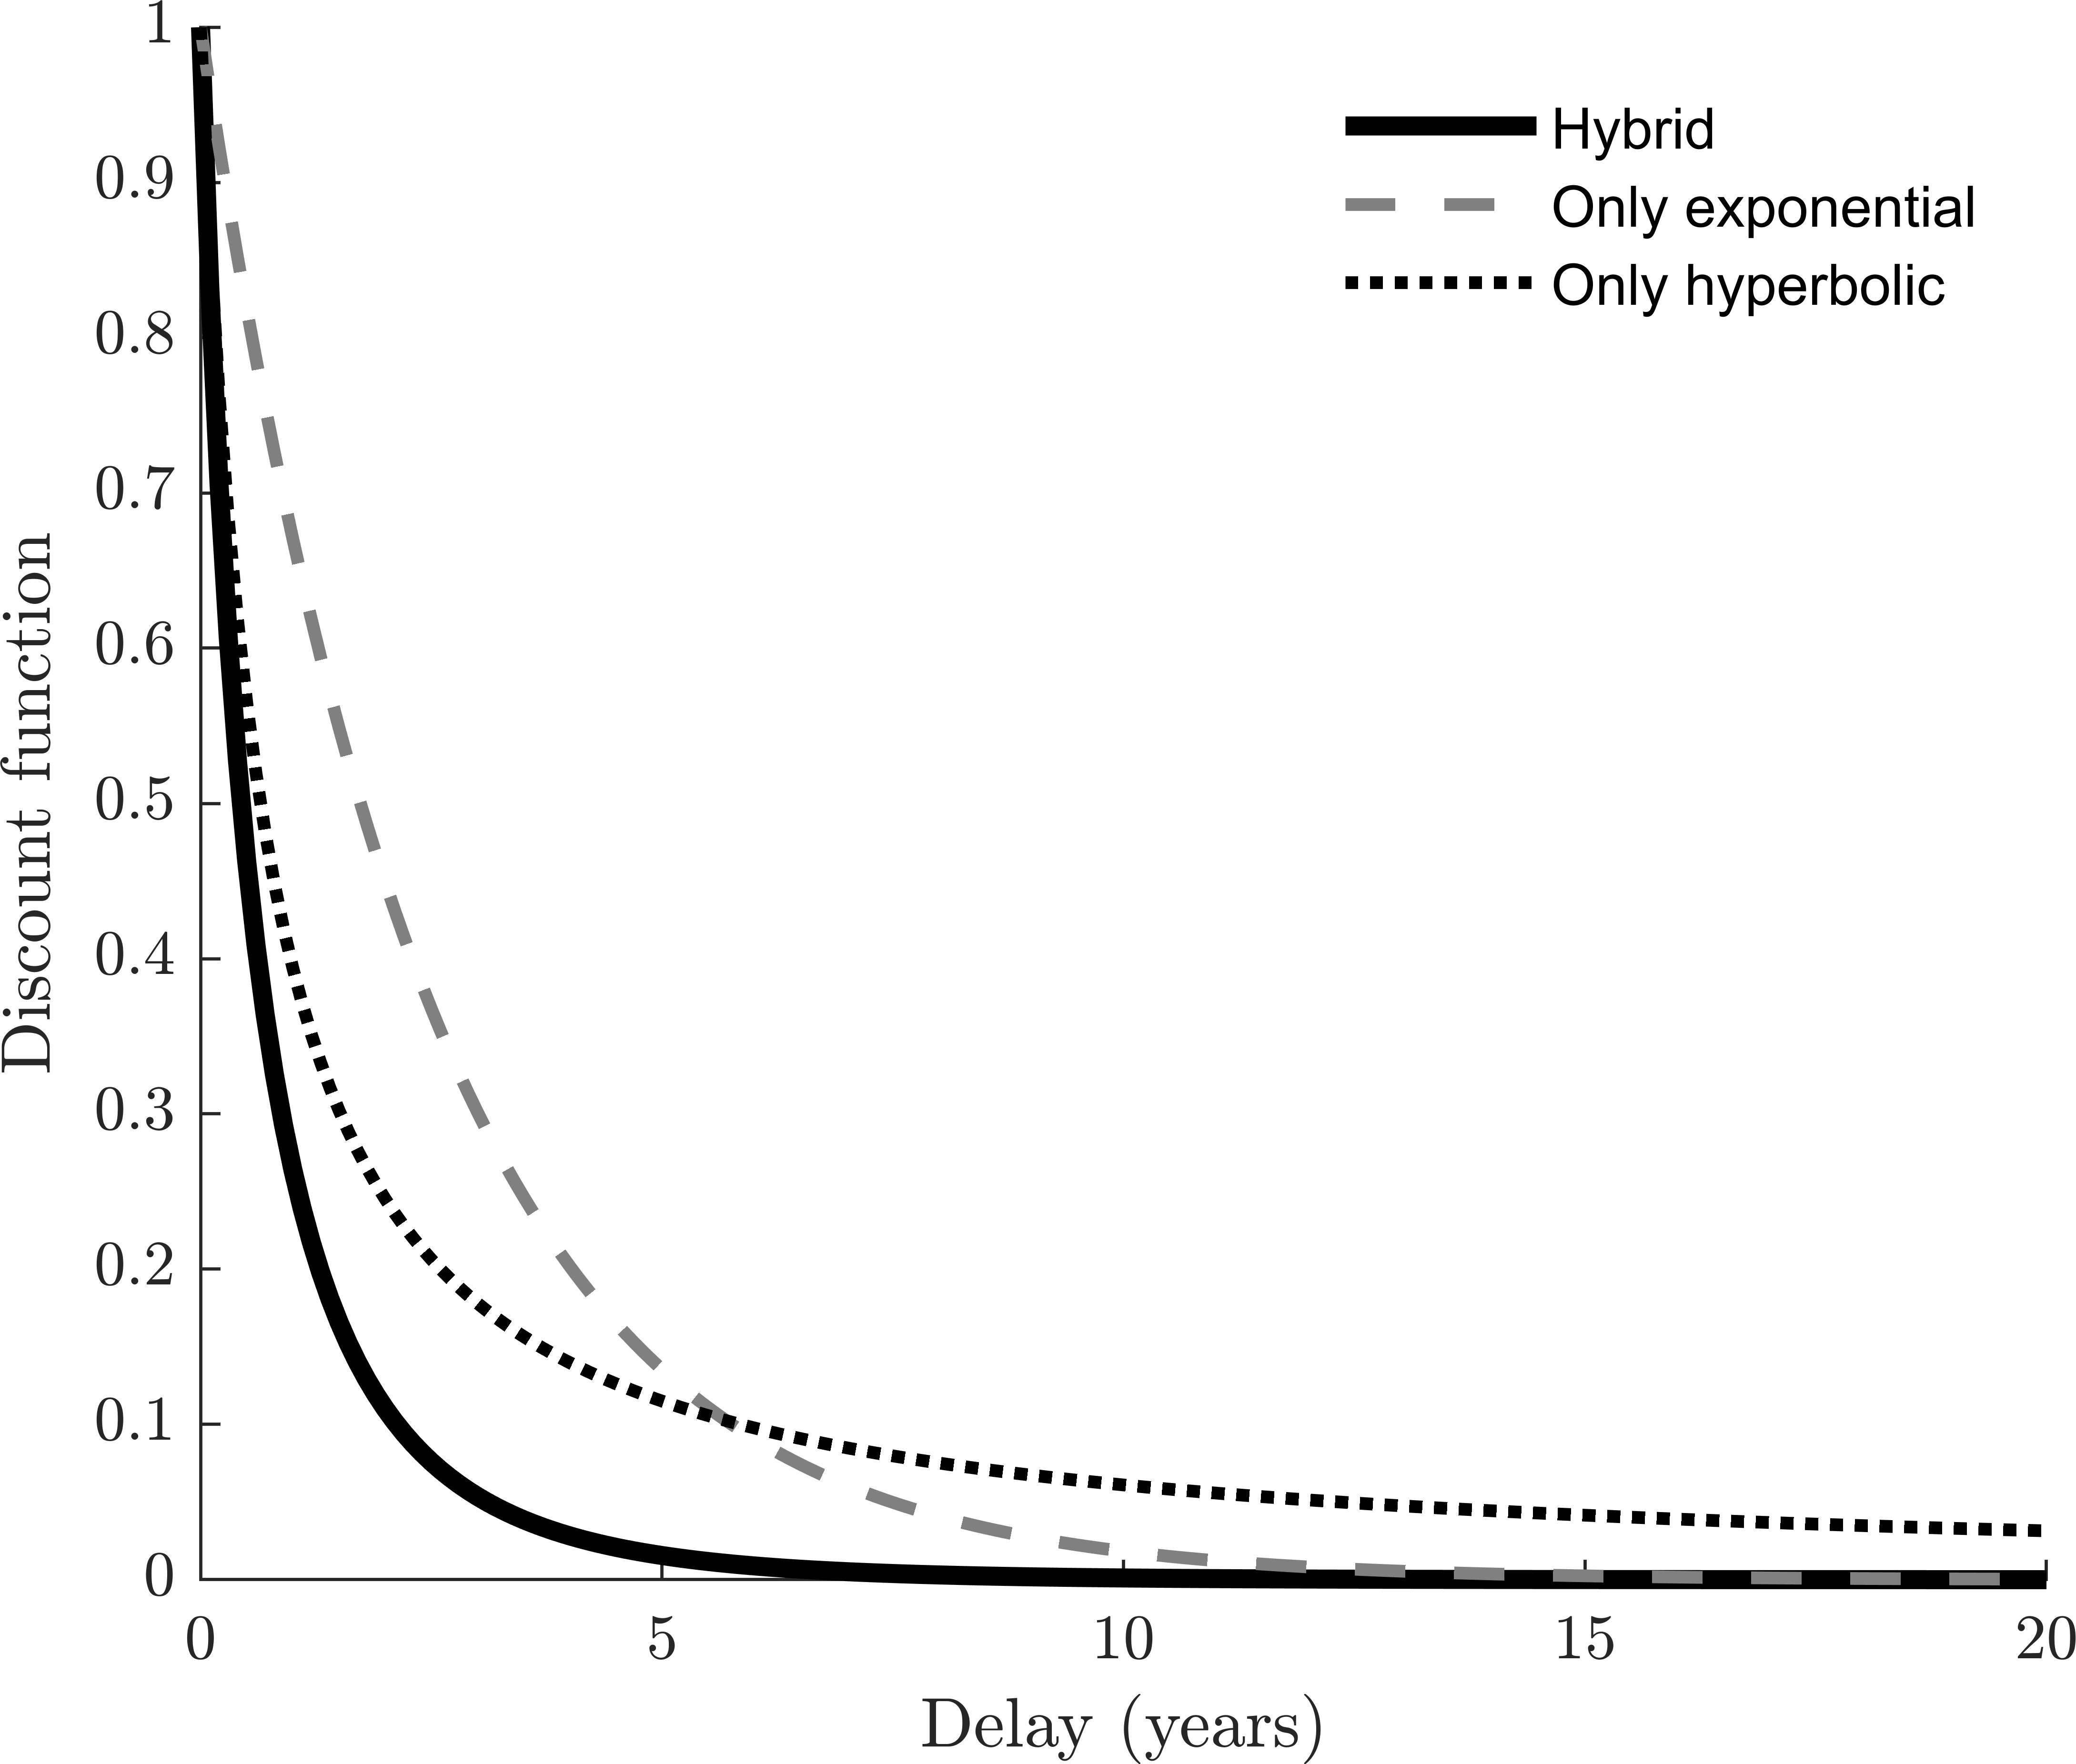
\includegraphics[width=0.7\textwidth]{./figures/caseD_delta_asymptotic.jpg} 
\end{frame}


\begin{frame}
Thank you for listening. I look forward to your comments. 

\includegraphics[width=0.7\textwidth]{./figures/yoda.jpg} 
\end{frame}

\end{document}